\chapter{Set Theory}


\section{Terminology}

A set is presented with a list of its elements surrounded by curly brackets. For instance, $\{1, 2, 3, 4\}$ is a way to present a set. A set may be presented as a family of objects satisfying a certain statement $P (n)$. For instance, $\{ n \, : \, n \text{ is an odd integer}\}$ would describe the set of odd integers $\{ \ldots , -3 , -1 , 1, 3, \ldots \}$.

Uppercase letters are usually used to denote sets and lowercase letters are used to denote an arbitrary element of a set. For example, $A = \{ 1 , 2, 3, 4\}$. The notation $a \in A$ is used to mean ``the element $a$ belongs to the set $A$''. The negation of $a \in A$ will be denoted by $x \not\in A$. This means the element $a$ does not belong to the set $A$. 

A \underline{reference set} or \underline{universal set} is a set $U$ containing all elements under consideration. For example, a sample space $S$ would be a universal set for an experiment. All the definitions below is based on the assumption of the existence of a universal set $U$.

\begin{definition}
The \underline{null set} is the set $\varnothing$ containing no element.
\end{definition}

\begin{definition}
If $A$ and $B$ are two sets, then $A$ is a \underline{subset} of $B$ if all the elements of the set $A$ belongs to the set $B$. We denote this by $A \subset B$. The family of all subsets, called the \underline{power set}, of a set $A$ is denoted by $2^A$.
\end{definition}

\underline{\textbf{Note:}} To prove that a set $A$ is a subset of $B$, the statement ``$\forall x \in A, x \in B$'' should hold. In other words, we have to prove that the statement ``$x \in A \Rightarrow x \in B$.

\begin{definition}
If $A$ and $B$ are two sets, then we say that $A$ is equal to $B$, denoted by $A = B$, if $A \subset B$ and $B \subset A$.
\end{definition}

In other words, all the elements of $A$ are the same as the elements of $B$.

\begin{definition}
If a set $A$ has a finite number of elements, then $\#A$ denotes the number of elements in $A$. 
\end{definition}

\section{Operations With Sets}

\begin{definition}
a) The set $A \cup B$ is the \underline{union} of $A$ and $B$. It is the set of elements from $A$ and from $B$. \underline{Note:} $A \cup S = S$. \\
b) The set $A \cap B$ is the set of all elements that are common to $A$ and $B$. It is called the \underline{intersection} of $A$ and $B$. \underline{Note:} $A \cap S = A$.
\end{definition}

\begin{figure}[ht]
    \centering
    \begin{subfigure}[b]{0.425\textwidth}
         \centering
         \begin{tikzpicture}
         \node (union) at (0, 0){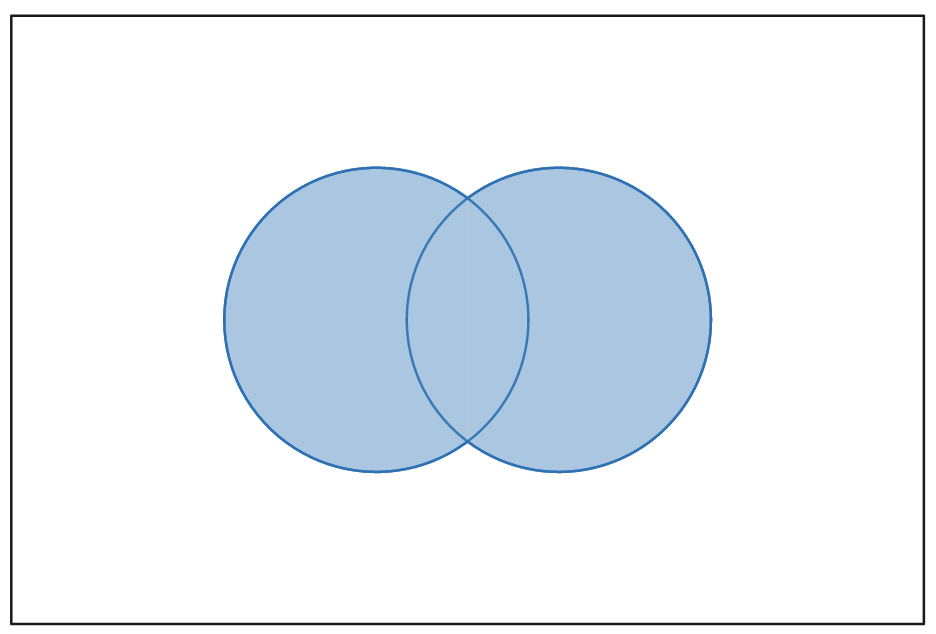
\includegraphics[scale=0.20]{union.png}};
         \draw (-3.5, 1.8)node{$U$};
         \draw (-1.5, 1)node{$A$};
         \draw (1.5, 1)node{$B$};
         \end{tikzpicture}\vspace{-8pt}
         \caption{Union}
     \end{subfigure}
     \begin{subfigure}[b]{0.425\textwidth}
        \centering
         \begin{tikzpicture}
         \node (union) at (0, 0){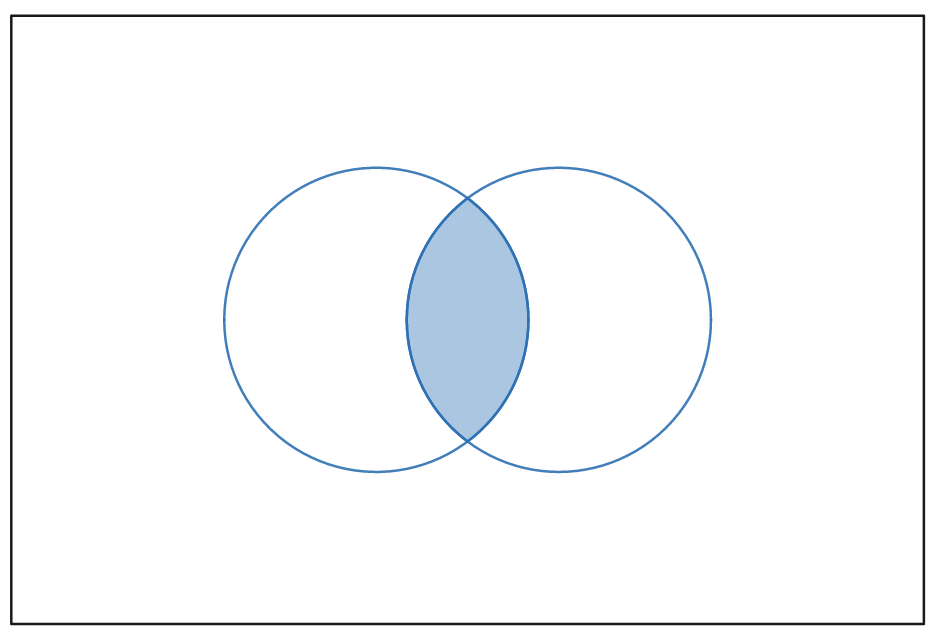
\includegraphics[scale=0.20]{intersection.png}};
         \draw (-3.5, 1.8)node{$U$};
         \draw (-1.5, 1)node{$A$};
         \draw (1.5, 1)node{$B$};
         \end{tikzpicture}\vspace{-8pt}
         \caption{Intersection}
     \end{subfigure}
    %\caption{Illustration of Union and Intersection Operations}
\end{figure}

\newpage


\underline{\textbf{Notes:}}
    \begin{itemize}
        \item Using the mathematical language from Appendix L, we can rewrite the union of $A$ and $B$ as followed: $A \cup B = \{ x \in U \, : \, x \in A \text{ or } x \in B\}$.
        \item Similarly, we can rewrite the intersection of $A$ and $B$ as followed: $A \cap B = \{ x \in U \, : \,  x \in A \text{ and } x \in B\}$.
    \end{itemize}

\begin{definition}
a) The \underline{complement} of a set is the new set $\overline{A}$ of all elements in $U$ that are not in $A$. Note that $A \cup \overline{A} = U$.\\
b) The \underline{set difference} of two sets $A$ and $B$ is the set $A \cap \overline{B}$. In other words, it is the set of elements that are in $A$, but not in $B$.
\end{definition}
    
    \begin{figure}[ht]
    \centering
     \begin{subfigure}[b]{0.45\textwidth}
        \centering
        \begin{tikzpicture}
         \node (union) at (0, 0){ 
\includegraphics[scale=0.22]{complement.png}};
         \draw (-3.8, 1.8)node{$U$};
         \draw (0, 0.75)node{$A$};
         \end{tikzpicture}\vspace{-8pt}
         \caption{Complement}
     \end{subfigure}
     \begin{subfigure}[b]{0.45\textwidth}
         \centering
          \begin{tikzpicture}
         \node (union) at (0, 0){ 
         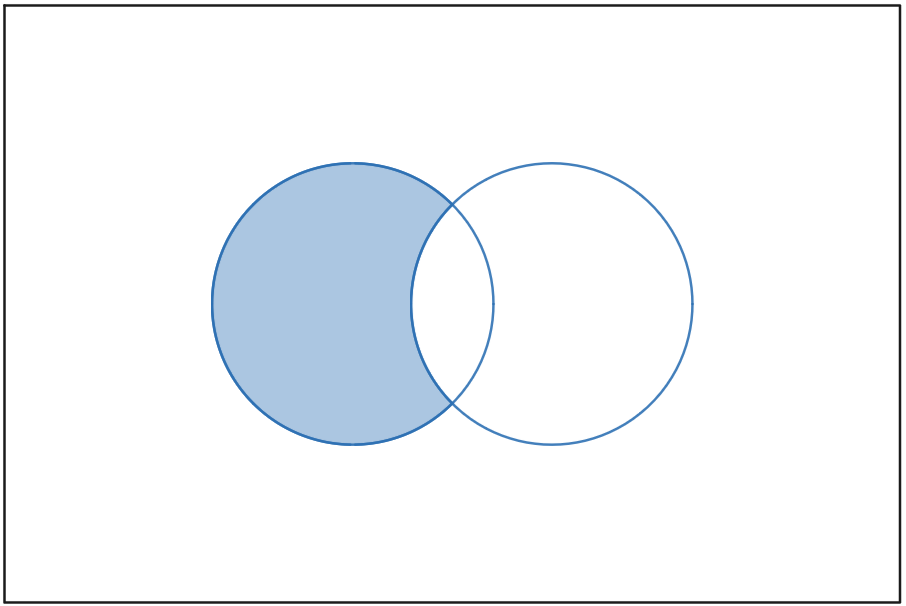
\includegraphics[scale=0.225]{difference.png}};
         \draw (-3.8, 1.8)node{$U$};
         \draw (-1.75, 1)node{$A$};
         \draw (1.75, 1)node{$B$};
         \end{tikzpicture}\vspace{-7pt}
         \caption{Difference}
     \end{subfigure}
    %\caption{Illustration of each operation}
    \end{figure}

    \underline{\textbf{Notes:}}
        \begin{itemize}
            \item We can rewrite the complement of a set $A$ as followed: $\overline{A} = \{ x \in U \, : \, x \not \in A \}$.
            \item We can rewrite the set difference of $A$ and $B$ as followed: $A \cap \overline{B} = \{ x \in U \, : \, x \in A \text{ and } x \not\in B \}$.
        \end{itemize}


    \begin{definition}
    Two sets, $A$ and $B$, are \underline{disjoint} or \underline{mutually exclusive} if $A \cap B = \varnothing$.
    \end{definition}

    \begin{example}
    Let $U= \{ 1 , 2, 3, 4 , 5 \}$. The sets $A = \{ 1 , 2 \}$ and $B = \{ 3 \}$ are mutually exclusive because they have nothing in common, meaning $A \cap B = \varnothing$.
    \end{example}

\newpage 

\section{Important Laws for Set Algebra}
    
    \begin{theorem}
        \begin{enumerate}[label=\alph*)]
        \item Commutative laws:
            \begin{align*}
            A \cup B = B \cup A \quad \text{and} \quad A \cap B = B \cap A .
            \end{align*}
        \item The distributive laws:
            \begin{align}
            A \cap (B \cup C ) &= (A \cap B) \cup (A \cap C ) \\
            A \cup (B \cap C ) &= (A \cup B) \cap (A \cup C ) .
            \end{align}
        \end{enumerate}
    \end{theorem}
    \begin{proof}
    We will prove one of the commutative laws and one of the distributive laws. The other formulas are left as an exercise.

    \begin{enumerate}[label=\alph*)]
    \item To prove the equation $A \cup B = B \cup A$, we have to show (i)$A \cup B \subset B \cup A$ and; (ii)$B \cup A \subset A \cup B$. 
        \begin{enumerate}[label=(\roman*)]
        \item Assume $x \in A \cup B$. Then, $x \in A$ or $x \in B$ by definition of the union of sets. But, this is the same thing as writing $x \in B$ or $x \in A$ (the order of the presentation is unimportant). Therefore, the element $x$ belongs to $B \cup A$ by definition of the union of $B$ and $A$. 
        \item Now, assume $x \in B \cup A$. Then $x \in B$ or $x \in A$ from the definition of $B \cup A$. Since the order of the presentation is unimportant, $x \in A$ or $x \in B$. Therefore, $x \in A \cup B$ by definition of the union of $A$ and $B$. 
        \end{enumerate}
        Let's wrap this up. We just proved that $A \cup B \subset B \cup A$ and that $B \cup A \subset A \cup B$. From the definition of equality of sets, this means $A \cup B = B \cup A$.
    \item We prove the equation $A \cap (B \cup C) = (A \cap B) \cup (A \cap C)$. 
        \begin{enumerate}[label=(\roman*)]
        \item We start by proving that $A \cap (B \cup C) \subset (A \cap B) \cup (A \cap C)$. Assume $x \in A \cap (B \cup C)$. Then, by definition of the intersection of two sets, this means $x \in A$ and $x \in B \cup C$. By definition of the union of two sets, $x \in B \cup C$ implies that $x \in B$ or $x \in C$. Since $x$ belongs to $A$ in both cases, then if $x$ belongs to $B$, we conclude that $x$ belongs to $A \cap B$, but if $x$ belongs to $C$, we conclude that $x$ belongs to $A \cap C$. Therefore, $x$ belongs to $A \cap B$ or to $A \cap C$. By definition of the union, the element $x$ belongs to $(A \cap B) \cup (A \cap C)$. 
        \item Now we prove that $(A \cap B) \cup (A \cap C) \subset A \cap (B \cup C)$. Assume $x \in (A \cap B) \cup (A \cap C)$. Then, this means that $x$ belongs to $A \cap B$ or to $A \cap C$. The fact $x \in A \cap B$ implies that $x \in A$ and $x \in B$. The second fact that $x \in A \cap C$ implies that $x \in A$ and $x \in C$. Since $x$ belongs to $A$ in both cases, we see that $x \in A$ and $x$ belongs to $B$ or to $C$. In other words, the element $x$ belongs to $A$ and to $B \cup C$, which means that $x \in A \cap (B \cup C)$.
        \end{enumerate}
        From (i) and (ii), we can then conclude that $A \cap (B \cup C) = (A \cap B) \cup (A \cap C)$.
    \end{enumerate}
    \end{proof}

    \begin{theorem}
    De Morgan's laws:
        \begin{align*}
        \overline{A \cap B} = \overline{A} \cup \overline{B} \quad \text{ and } \quad \overline{A \cup B} = \overline{A} \cap \overline{B} .
        \end{align*}
    \end{theorem}
    \begin{proof}
    We only prove the first equation and leave the proof of the second one as an exercise. 

    Suppose $x \in \overline{A \cap B}$. From the definition of the complement of a set, $x \not\in A \cap B$. this means that $x$ does not belong to $A \cap B$. We have to negate the definition of intersection. We have $x \in A \cap B$ when $x \in A$ \textit{and} $x \in B$. The negation is $x \not\in A$ or $x \not\in B$. Therefore, $x \in \overline{A}$ or $x \in \overline{B}$. From the definition of the union of two sets, we see that $x \in \overline{A} \cup \overline{B}$.

    Now, assume $x \in \overline{A} \cup \overline{B}$. This means that $x \not\in A$ or $x \not\in B$. From the last paragraph, this last statement is the negation of $x \in A \cap B$. Therefore, $x \not\in A \cap B$. In other words, $x$ belongs to $\overline{A \cap B}$. 

    We can then conclude that $\overline{A \cap B} = \overline{A} \cup \overline{B}$. 
    \end{proof}

\begin{comment}
\section{Problems Set}

\subsection*{Terminology}

\begin{problem}
Let $U = \{1 , 2, 3, 4, 5 \}$, $A = \{ 1 , 2 \}$, and $B = \{ 1 , 2, 3\}$. Show that $A \subset B$.
\end{problem}

\begin{problem}
Let $U = \{ 1 , 2, 3, 4\}$. Show that $U$ has $2^4$ subsets. \underline{Bonus:} In general, show that if $U$ has a finite number of elements, then $U$ has $2^{(\#U)}$ subsets.
\end{problem}

\begin{problem}
Show that if $A$ is a set, then $\varnothing \subset A$.
\end{problem}

\begin{problem}
Let $A$, $B$, and $C$ be subsets of a universal set $U$. Show that if $A \subset B$ and $B \subset C$, then $A \subset C$.
\end{problem}

\subsection*{Operations With Sets}

\begin{problem}
Let $A$ and $B$ be two subsets of a universal set $U$.
    \begin{enumerate}[label=\alph*)]
        \item Show that $A \cap B \subset A$.
        \item Show that $A \subset A \cup B$.
        \item Show that if $A \subset B$, then $A \cup B = B$.
        \item Show that if $A \subset B$, then $A \cap B = A$.
    \end{enumerate}
\end{problem}

\begin{problem}
Let $A$ and $B$ be two subsets of a universal set $U$.
    \begin{enumerate}[label=\alph*)]
        \item Show that $A \cup \overline{A} = U$.
        \item Show that if $A \subset B$, then $\overline{B} \subset \overline{A}$.
    \end{enumerate}
\end{problem}

\begin{problem}
Let $A = \{ n \, : \, n \text{ is an odd integer}\}$ and let $B = \{ n \, : \, n \text{ is an even integer}\}$. Show that $A \cap B = \varnothing$. \textit{[Hint: To prove $A \cap B \subset \varnothing$, use the method of proof by contradiction.]}
\end{problem}

\subsection*{Important Laws For Set Algebra}

\begin{problem}
Let $A$, $B$, and $C$ be subsets of a universal set $U$.
    \begin{enumerate}[label=\alph*)]
        \item Prove that $A \cap B = B \cap A$.
        \item Prove that $A \cup (B \cap C) = (A \cup B) \cap (A \cup C)$.
        \item $\overline{A \cup B} = \overline{A} \cap \overline{B}$.
    \end{enumerate}
\end{problem}




\section{Solutions to Problems Set}
\setcounter{problem}{0} 

\subsection*{Terminology}

\begin{problem}
Let $x \in A$. Then either $x = 1$ or $x = 2$. When $x = 1$, we see that $1 \in B$, so $x \in B$. When $x = 2$, we see that $2 \in B$, so that $x \in B$. Therefore, $\forall x \in A$, $x \in B$ and $A \subset B$.
\end{problem}

\begin{problem}
The power set of $U$ is 
\begin{align*}
2^U &= \{ \varnothing , \{ 1 \} , \{ 2 \} , \{ 3 \} , \{4 \} , \{ 1 , 2\} , \{ 1 , 3\} , \{ 1 , 4 \} , \{ 2 , 3\} , \{ 2, 4\} , \{ 3 , 4 \} , \\
& \phantom{=} \, \, \, \,  \{ 1 , 2, 3 \} , \{ 1 , 2, 4 \} , \{ 1 , 3 , 4, \} , \{ 2 , 3, 4, \} , U \} .
\end{align*}
Counting the number of subsets in the power set will give the total number of subsets of $U$. There are 16 items in the power set $2^U$ and $16 = 2^4$.

In general, define a subset $A$ of $U$ as a function $f_A : U \ra \{ 0 , 1\}$ in the following way:
    \begin{align*}
    f_A (x) = \left\{ \begin{matrix}
    1 & x \in A \\
    0 & x \not\in A .\end{matrix} \right. 
    \end{align*} 
Then the number of subsets of $U$ will be determined by the number of functions from $U$ into $\{ 0 , 1\}$. There are $2^{\#U}$ such functions because for each element $x \in U$, you have two possible choice for $f_A (x)$.
\end{problem}

\begin{problem}
By definition of $\varnothing \subset A$, we have to show that if $x \in \varnothing$, then $x \in A$. However, the assumption is always false and therefore the implication $x \in \varnothing \Rightarrow x \in A$ is always true. Thus $\varnothing \subset A$.
\end{problem}

\begin{problem}
Let $x \in A$. Since $A \subset B$, then $x \in B$. Now, since $B \subset C$, then $x \in C$. The element $x$ was arbitrarily chosen, so $A \subset C$.
\end{problem}

\subsection*{Operations With Sets}

\begin{problem}
Let $A$ and $B$ be two subsets of a universal set $U$.
    \begin{enumerate}[label=\alph*)]
        \item Let $x \in A \cap B$. By definition of intersection, we then have $x \in A$ and $x \in B$. In particular, we have $x \in A$. Since $x$ was arbitrary, then $A \cap B \subset A$.
        \item Let $x \in A$. Then the disjunction statement ``$x \in A$ or $x \in B$'' is true because $x \in A$ is assume to be true. Therefore, $x \in A \cup B$ by definition of the union of two sets. Since $x$ was arbitrary, then $A \subset A \cup B$.
        \item Assume that $A \subset B$. 
        We start by showing that $A \cup B \subset B$. If $x \in A \cup B$, then $x \in A$ or $x \in B$ by definition of union. Two cases:
            \begin{itemize}
            \item If $x \in A$, then $x \in B$ because $A \subset B$.
            \item If $x \in B$, then $x \in B$ (tautology).
            \end{itemize}
        In both cases, we obtain that $x \in B$. Since $x$ was arbitrary, we have $A \cup B \subset B$. We now show that $B \subset A \cup B$. From part b), we have $B \subset B \cup A$. Since $B \cup A = A \cup B$, we obtain $B \subset A \cup B$.

        Since $A \cup B \subset B$ and $B \subset A \cup B$, we have $A \cup B = B$.
        \item Assume that $A \subset B$. Let $x \in A \cap B$. Then $x \in A$ and $x \in B$. In particular $x \in A$. So $A \cap B \subset A$. Let $x \in A$. Then $x \in B$ also because $A \subset B$. Therefore $x \in A$ and $x \in B$ and so $x \in A \cap B$. So $A \subset A \cap B$. Since $A \cap B \subset A$ and $A \subset A \cap B$, we get $A \cap B = A$.
    \end{enumerate}
\end{problem}

\begin{problem}
Let $A$ and $B$ be two subsets of a universal set $U$.
    \begin{enumerate}[label=\alph*)]
        \item We have to show that $A \cup \overline{A} \subset U$ and $U \subset A \cup \overline{A}$. 

        Let $x \in A \cup \overline{A}$. There are two cases because of the definition of union:
            \begin{itemize}
                \item If $x \in A$, then $x \in U$ because $A \subset U$.
                \item If $x \in \overline{A}$, then $x \in U$ because $\overline{A} \subset U$.
            \end{itemize}
        Each case implies that $x \in U$. Therefore, $A \cup \overline{A} \subset U$.

        Let $x \in U$. Then $x \in A$ or $x \not\in A$ which implies that $x \in A \cup \overline{A}$. Therefore $U \subset A \cup \overline{A}$. 
        \item Assume that $A \subset B$. Let $x \in \overline{B}$. We will argue by contradiction. Suppose that $x \in A$. By assumption, this implies that $x \in B$. But $x \in \overline{B}$. In other words, $x \in B$ and $x \not\in B$. This is not possible and therefore $x \in \overline{A}$. [\textit{Note: You can also take the contrapositive for a direct proof! The contrapositive of $A \subset B$ is $x \not\in B \Rightarrow x \not\in A$ which is equivalent to $x \in \overline{B} \Rightarrow x \in \overline{A}$.}]
    \end{enumerate}
\end{problem}

\begin{problem}
Since $\varnothing \subset A \cap B$, we only need to prove that $A \cap B \subset \varnothing$. We will argue by contradiction. For $A \cap B$ to not be a subset of $\varnothing$, it must contain at least one element. So, assume that $x \in A \cap B$. This implies that $x \in A$ and $x \in B$. By definition of $A$, $x$ is an odd integer. By definition of $B$, $x$ is also an even integer. But an integer can't be odd and even at the same time by Example \ref{Ex:NoIntIsOddAndEven} and this is a contradiction. Therefore, $A \cap B \subset \varnothing$.

Since $\varnothing \subset A \cap B$ and $A \cap B \subset \varnothing$, we conclude that $A \cap B = \varnothing$.
\end{problem}

\subsection*{Important Laws For Set Algebra}

\begin{problem}
Let $A$, $B$, and $C$ be subsets of a universal set $U$.
    \begin{enumerate}[label=\alph*)]
        \item We have
            \begin{align*}
            x \in A \cap B & \iff x \in A \text{ and } x \in B \quad \text{[Definition of $A \cap B$]}\\
            & \iff x \in B \text{ and } x \in A \quad \text{[Order of words don't matter]} \\
            & \iff x \in B \cap A \quad \text{[Definition of $B \cap A$]}
            \end{align*}
        \item We start by showing that $A \cup (B \cap C) \subset (A \cup B) \cap (A \cup C)$. Let $x \in A \cup (B \cap C)$. Then by definition of the union, we have $x \in A$ or $x \in B \cap C$. The fact $x \in B \cap C$ implies that $x \in B$ and $x \in C$. In particular, $x \in B$. Combined with $x \in A$, we obtain $x \in A$ or $x \in B$. Similarly, we obtain $x \in A$ or $x \in C$. We can then create the conjunction of ``$x \in A$ or $x \in B$'' with ``$x \in A$ or $x \in C$'', that is $(x \in A \vee x \in B) \wedge (x \in A \vee x \in C)$. Using the definition of union, the last statement is rewritten as $(x \in A \cup B) \wedge (x \in A \cup C)$. From the definition of intersection, we can rewrite the last statement as $x \in (A \cup B) \cap (A \cup C)$. 

        To show that $(A \cup B) \cap (A \cup C) \subset A \cup (B \cap C)$ is similar. We just start from the end of the previous paragraph and make our way back to the first sentence of the paragraph (so read the last paragraph from the last sentence to the first sentence to obtain the proof). 

        Therefore, we just proved equality between the two sets.
        \item We have
            \begin{align*}
             x \in \overline{A \cup B} & \iff x \not\in A \cup B \\
             & \iff x \not\in A \wedge x \not\in B \quad \text{[Negation of $A \cup B$]} \\
             & \iff x \in \overline{A} \wedge x \in \overline{B} \quad \text{[Definition of complement]} \\
             & \iff x \in \overline{A} \cap \overline{B} \quad \text{[Definition of intersection]}.
             \end{align*}
        Therefore, $\overline{A \cup B} = \overline{A} \cap \overline{B}$.
    \end{enumerate}
\end{problem}

\end{comment}